\documentclass{article}
%%%%%%% PREAMBLE %%%%%%%
%BEGIN_FOLD
%%%%% PACKAGES
\usepackage{amsmath}
\usepackage{amssymb}
\usepackage{amsthm}
\usepackage{cabin} % section title font
\usepackage[default]{cantarell} % default font
\usepackage{capt-of}
\usepackage{circuitikz}
\usepackage[shortlabels]{enumitem}
\usepackage{fancyhdr}
\usepackage{graphicx}
\usepackage{hyperref}
\usepackage{mathtools}
\usepackage[framemethod=TikZ]{mdframed}
\usepackage[scr]{rsfso} % power set symbol
\usetikzlibrary{shapes}
\usepackage{tasks} % vaguely remember this being important for something...?
\usepackage{tikz} % diagrams
\usepackage{titlesec}
\usepackage{thmtools}
\usepackage{varwidth}
\usepackage{verbatim} % longer comments
\usepackage{xcolor}
%%%%%

%%%%% COLOURS
\definecolor{darkgreen}{HTML}{19A514}
\definecolor{lightgreen}{HTML}{9DFF9A}
\definecolor{darkblue}{HTML}{3E5FE4}
\definecolor{lightblue}{HTML}{BCDEFF}
\definecolor{darkred}{HTML}{CC3333}
\definecolor{lightred}{HTML}{FFA9A9}
\definecolor{darkpurple}{HTML}{A933CD}
\definecolor{lightpurple}{HTML}{F0BAFF}
\definecolor{darkyellow}{HTML}{D2D22A}
\definecolor{lightyellow}{HTML}{FFFFAE}
\definecolor{hyperlinkblue}{HTML}{3366CC}
%%%%%

%%%%% PAGE SETUP
% BASIC %
\setlength\parindent{0pt} % paragraph indentation
\setlength{\parskip}{5pt} % spacing between paragraphs
\usepackage[margin=1in]{geometry} % margin size

% HEADER/FOOTER %
\pagestyle{fancy}
\fancyhf{}
\fancyfoot[R]{\thepage} % page number on bottom right
\fancyhead[R]{\textit{\leftmark}} % section title
\renewcommand{\headrulewidth}{0pt} % removing horizontal line at the top

% HYPERLINK FORMATTING %
\hypersetup{
	colorlinks,    
	linkcolor=hyperlinkblue,
	urlcolor=hyperlinkblue,
	pdftitle={...},
	pdfauthor={Michael Pham},
}

%%%%%

%%%%% ENVIRONMENTS STYLES
% SOLUTION ENVIRONMENT %
\newenvironment{solution}{\begin{proof}[Solution]}{\end{proof}}

% PURPLE BOX %
\declaretheoremstyle[
mdframed={
	backgroundcolor=lightpurple,
	linecolor=darkpurple,
	rightline=false,
	topline=false,
	bottomline=false,
	linewidth=2pt,
	innertopmargin=8pt,
	innerbottommargin=8pt,
	innerleftmargin=8pt,
	leftmargin=-2pt,
	skipbelow=2pt,
	nobreak
},
headfont=\normalfont\bfseries\color{darkpurple}
]{purplebox}

% GREEN BOX %
\declaretheoremstyle[
mdframed={
	backgroundcolor=lightgreen,
	linecolor=darkgreen,
	rightline=false,
	topline=false,
	bottomline=false,
	linewidth=2pt,
	innertopmargin=8pt,
	innerbottommargin=8pt,
	innerleftmargin=8pt,
	leftmargin=-2pt,
	skipbelow=2pt,
	nobreak
},
headfont=\normalfont\bfseries\color{darkgreen}
]{greenbox}

% YELLOW BOX %
\declaretheoremstyle[
mdframed={
	backgroundcolor=lightyellow,
	linecolor=darkyellow,
	rightline=false,
	topline=false,
	bottomline=false,
	linewidth=2pt,
	innertopmargin=8pt,
	innerbottommargin=8pt,
	innerleftmargin=8pt,
	leftmargin=-2pt,
	skipbelow=2pt,
	nobreak
},
headfont=\normalfont\bfseries\color{darkyellow}
]{yellowbox}

% BLUE BOX %
\declaretheoremstyle[
mdframed={
	backgroundcolor=lightblue,
	linecolor=darkblue,
	rightline=false,
	topline=false,
	bottomline=false,
	linewidth=2pt,
	innertopmargin=8pt,
	innerbottommargin=8pt,
	innerleftmargin=8pt,
	leftmargin=-2pt,
	skipbelow=2pt,
	nobreak
},
headfont=\normalfont\bfseries\color{darkblue}
]{bluebox}

% RED BOX %
\declaretheoremstyle[
mdframed={
	backgroundcolor=lightred,
	linecolor=darkred,
	rightline=false,
	topline=false,
	bottomline=false,
	linewidth=2pt,
	innertopmargin=8pt,
	innerbottommargin=8pt,
	innerleftmargin=8pt,
	leftmargin=-2pt,
	skipbelow=2pt,
	nobreak
},
headfont=\normalfont\bfseries\color{darkred}
]{redbox}
%%%%%

%%%%% ENVIRONMENTS
% PURPLE BOXES (theorems, propositions, lemmas, and corollaries) %
\declaretheorem[style=purplebox,name=Theorem,within=section]{thm}
\declaretheorem[style=purplebox,name=Theorem,sibling=thm]{theorem}
\declaretheorem[style=purplebox,name=Theorem,numbered=no]{thm*, theorem*}
\declaretheorem[style=purplebox,name=Proposition,sibling=thm]{prop, proposition}
\declaretheorem[style=purplebox,name=Proposition,numbered=no]{prop*, proposition*}
\declaretheorem[style=purplebox,name=Lemma,sibling=thm]{lem, lemma}
\declaretheorem[style=purplebox,name=Lemma,numbered=no]{lem*, lemma*}
\declaretheorem[style=purplebox,name=Corollary,sibling=thm]{cor, corollary}
\declaretheorem[style=purplebox,name=Corollary,numbered=no]{cor*, corollary*}

% GREEN BOXES (definitions) %
\declaretheorem[style=greenbox,name=Definition,sibling=thm]{definition, defn}
\declaretheorem[style=greenbox,name=Definition,numbered=no]{definition*, defn*}

% BLUE BOXES (problems) %
\declaretheorem[style=bluebox,name=Problem,numberwithin=section]{homework, hw}
\declaretheorem[style=bluebox,name=Problem,numbered=no]{homework*, hw*}

% RED BOXES %
\declaretheorem[style=redbox,name=Remark,sibling=thm]{remark, rmk}
\declaretheorem[style=redbox,name=Remark, numbered=no]{remark*, rmk*}
\declaretheorem[style=yellowbox,name=Warning,sibling=thm]{warn}
\declaretheorem[style=yellowbox,name=Warning,numbered=no]{warn*}
%%%%%

%%%%% PROOF FORMATTING
\renewcommand\qedsymbol{$\blacksquare$}
%%%%%

%%% CUSTOM COMMANDS
% basic %
\newcommand{\Mod}[1]{\ (\mathrm{mod}\ {#1})}
\renewcommand{\gcd}[1]{\ \text{gcd}\ ({#1})}
\newcommand{\floor}[1]{\left\lfloor{#1}\right\rfloor}
\newcommand{\ceil}[1]{\left\lceil{#1}\right\rceil}
\newcommand{\norm}[1]{\left\lVert{#1}\right\rVert}

% logic %
\newcommand*\xor{\oplus}
\newcommand{\all}{\forall}
\newcommand{\bland}{\bigwedge}
\newcommand{\blor}{\bigvee}
\newcommand*{\defeq}{\mathrel{\rlap{\raisebox{0.3ex}{$\m@th\cdot$}}\raisebox{-0.3ex}{$\m@th\cdot$}}=} \makeatother

% matrices %
\newcommand\aug{\fboxsep=- \fboxrule\!\!\!\fbox{\strut}\!\!\!}\makeatletter 

% sets %
\newcommand{\CC}{\mathbb{C}}
\newcommand{\NN}{\mathbb{N}}
\newcommand{\QQ}{\mathbb{Q}}
\newcommand{\RR}{\mathbb{R}}
\newcommand{\ZZ}{\mathbb{Z}}

% title %
\newcommand{\mytitle}[2]{%
	\title{#1}
	\author{Michael Pham}
	\date{#2}
	\maketitle
	\newpage
	\tableofcontents
	\newpage
}
%%%

%%% REDEFINING COMMANDS
\let\oldint\int
\renewcommand{\int}[2]{\oldint\limits_{#1}^{#2}}
\let\oldprod\prod
\renewcommand{\prod}[2]{\oldprod\limits_{#1}^{#2}}
\let\oldsum\sum
\renewcommand{\sum}[2]{\oldsum\limits_{#1}^{#2}}
%%%

\newcommand*\circled[1]{\tikz[baseline=(char.base)]{
		\node[shape=circle,draw,inner sep=1](char) {#1};}}
%%%%%
%END_FOLD
%%%%%

\begin{document}
\mytitle{CS70 Homework 3}{Spring 2023}
\setcounter{section}{-1}
\section{Sundry}
For this week's homework, I did not work with anybody when coming up with my solutions. However, I did provide hints to people as to how I approached the problems in the Discord server.

\newpage

\section{Planarity and Graph Complements}
Let $G = (V, E)$ be an undirected graph.  We define the complement of $G$ as $\overline{G} = (V, \overline{E})$ where $\overline{E} = \{(i,j) \mid i,j \in V, i \neq j\} - E$; that is, $\overline{G}$ has the same set of vertices as $G$, but an edge $e$ exists is $\overline{G}$ if and only if it does not exist in $G$.

\begin{hw}
	Suppose $G$ has $v$ vertices and $e$ edges.  How many edges does $\overline{G}$ have?
\end{hw}
\begin{solution}
	For a graph $G$ with $v$ vertices and $e$ edges, $\overline{G}$ will have $v$ vertices as well by definition.
	
	For the number of edges, observe that for $v$ vertices, we have $\binom{v}{2}=\frac{v(v-1)}{2}$ unordered pairs of vertices, which is the number of edges. Then, from here, we see that the number of edges for $\overline{G}$, given that $G$ has $e$ edges, is $\frac{v(v-1)}{2}-e$.
	
	Thus, we have that $\overline{G}$ has $v$ vertices and $\frac{v(v-1)}{2}-e$ edges.
\end{solution}

\begin{hw}
	Prove that for any graph with at least 15 vertices, $G$ being planar implies that $\overline{G}$ is non-planar.
\end{hw}
\begin{solution}
	We shall proceed by contradiction.
	
	Suppose that we have a planar graph $G$ with $v \geq 15$ vertices and edges $e$, and let us suppose that $\overline{G}$ exists and is planar.
	
	Now, observe that if a graph is planar, we have that $e \leq 3v - 6$. 
	
	From here, we see that by definition, $\overline{G}$ has $\frac{v(v-1)}{2}-e$ edges, and $v \geq 15$ vertices. Then, as $\overline{G}$ is planar by assumption, we see that $\frac{v(v-1)}{2}-e \leq 3v - 6$.
	
	Then, if we combine the two inequalities, we get:
	\begin{align*}
		\frac{v(v-1)}{2} &\leq 6v - 12 \\
		v(v-1) &\leq 12v - 24 \\
		v^{2} - 13v + 24 &\leq 0 \\
		(v-12)(v-1) &\leq 0
	\end{align*}

	Then, we see that this implies that $v \leq 12$. However, this results in a contradiction, as we assumed that $\overline{G}$ has $v \geq 15$ edges.
	
	Therefore, we can conclude that $\overline{G}$ must be non-planar.
\end{solution}

\begin{hw}
	Now consider the converse of the previous part, i.e., for any graph $G$ with at least 15 vertices, if $\overline{G}$ is non-planar, then $G$ is planar. Construct a counterexample to show that the converse does not hold.
\end{hw}
\begin{solution}
	Let us suppose that a graph $\overline{G}$ is made of four $K_{5}$ graphs joined together. Then, we observe that it has $16 \geq 15$ vertices, and is non-planar (by Kuratowski's Theorem). From here, we observe that the number of edges that $\overline{G}$ has is $4(10) = 40$. Then, we observe that the number of edges for $G$ is $e = \frac{16(15)}{2}-40 = 80$ edges. However, we see that $80 = e \not\leq 3v-6 = 3(16)-6 = 42$. Therefore, we see that $G$ is non-planar as well.
	
	Therefore, we observe that the converse isn't necessarily true.
\end{solution}

\newpage

\section{Touring Hypercube}
In the lecture, you have seen that if $G$ is a hypercube of dimension $n$, then
\begin{itemize}
	\item The vertices of $G$ are the binary strings of length $n$.
	\item $u$ and $v$ are connected by an edge if they differ in exactly one bit location.
\end{itemize}

A \emph{Hamiltonian tour} of a graph is a sequence of vertices
$v_0, v_1, \ldots, v_k$ such that:
\begin{itemize}
	\item Each vertex appears exactly once in the sequence.
	\item Each pair of consecutive vertices is connected by an edge.
	\item $v_0$ and $v_k$ are connected by an edge.
\end{itemize}

\begin{hw}
	Show that a hypercube has an Eulerian tour if and only if $n$ is even.
\end{hw}
\begin{solution}
	In order to prove the claim, we must show that it holds true in both directions.
	
	First, we will begin with the forward direction.
	\begin{proof}[If]
		We shall proceed by contradiction
		
		Let us suppose that a hypercube $G$ of dimension $n$ has an Eulerian tour, where $n$ is odd.
		
		From here, recall that the degree of each vertex in a hypercube is $n$ as $n$ bit positions can be flipped in any $x \in \left\{  0,1\right\}^{2n}$. Then, this means that all of $G$'s vertices are of odd degree. However, as a graph has an Eulerian tour if and only if it is even degree, we observe that $G$ can't have an Eulerian tour, contradicting our original assumption.
		
		Therefore, we can conclude that if $G$ has an Eulerian tour, then $n$ must be even.
	\end{proof}

	Next, we will show the other direction.
	\begin{proof}[Only if]
		We shall proceed by direct proof.
		
		Let us suppose that a hypercube $G$ is of dimension $n$, where $n$ is even. From here, we observe that each vertex of the hypercube must have degree $n$ as well. 
		Since all vertices are of even degree, then we know that $G$ must have an Eulerian tour.
		
		Therefore, we can conclude that if for a hypercube $G$, $n$ is even then $G$ has an Eulerian tour.
	\end{proof}

	As we have proved both direction, we can thus conclude that $G$ has an Eulerian tour if and only if $n$ is even.
\end{solution}

\begin{hw}
	Show that every hypercube has a Hamiltonian tour. 
\end{hw}
\begin{solution}
	We shall proceed by induction.
	
	\textbf{\underline{Base Case}}: First, for a hypercube $G$ of dimension $n=0$, we observe that as it's only a single vertex, then a Hamiltonian graph exists, with the sequence simply being $v_{0}$, the vertex itself.
	
	First, for a hypercube $G$ of dimension $n=1$, we observe that there is a Hamiltonian tour as we can go from $0$ to $1$, then back to $0$ again.
	
	For a hypercube $G$ of dimension $n=2$, we observe that there's a Hamiltonian tour by going from $00$ to $01$ to $11$ to $10$ and then back to $00$. Thus, we have a Hamiltonian tour as desired.
	
	\textbf{\underline{Induction Hypothesis}}: Suppose that for a hypercube $G$ of dimension $n=k$, our claim holds true.
	
	\textbf{\underline{Inductive Step}}: Now we want to prove our induction hypothesis for $n=k+1$. Let $H$ be a $k$ dimensional hypercube with vertices $\left\{ v_{0}, \ldots, v_{2^{k}-1}\right\}$. By our induction hypothesis, we know that $H$ has a Hamiltonian tour. Now, observe that $G$ can be constructed by having two copies of $H$ with edges connecting each matching pair of vertices together (meaning that, for example, there is an edge that connects $H_{0}$ to $H'_{0}$, where $H_{0}$ and $H'_{0}$ are the vertices of all zeroes of $n$ length).
	
	From here we see that if we first start at $H_{0}$ and go to $H'_{0}$ by going through all the vertices starting with $0$. Then, at $H'_{0}$, we know that there is an edge connecting it to $H'_{1}$ (which is the vertex starting with $1$, followed by all zeroes). From here, we can go from $H'_{1}$ to $H_{1}$ by going through all vertices starting with $1$. Then, at $H_{1}$, we know that we can go back to $H_{0}$. Thus, this path described forms a Hamiltonian tour.
	
	Therefore, by mathematical induction, we can conclude that every hypercube $G$ has a Hamiltonian tour.
\end{solution}

\newpage

\section{Binary Trees}
You may have seen the recursive definition of binary trees from previous classes. Here, we define binary trees in graph theoretic terms as follows (\textbf{Note:} here we will modify the definition of leaves slightly for consistency). 
\begin{itemize}
	\item A binary tree of height $> 0$ is a tree where exactly one vertex, called the \textbf{root}, has degree $2$, and all other vertices have degrees $1$ or $3$. Each vertex of degree $1$ is called a \textbf{leaf}. The \textbf{height} $h$ is defined as the maximum length of the path between the root and any leaf.
	\item A binary tree of height $0$ is the graph with a single vertex. The vertex is both a leaf and a root.
\end{itemize}

\begin{hw}
	Let $T$ be a binary tree of height $> 0$, and let $h(T)$ denote it's height. Let $r$ be the root in $T$ and $u$ and $v$ be it's neighbors. Show that removing $r$ from $T$ will result in two binary trees, $L,R$ with roots $u$ and $v$ respectively. Also, show that $h(T) = \max(h(L),h(R)) + 1$.
\end{hw}
\begin{solution}
	We shall proceed by induction on the height $h$ of a tree $T$.
	
	\textbf{\underline{Base Case}}: Consider the tree $T$ of height $1$. $T$ will have a root $r$ along with two vertices connected to it: $u$ and $v$. Now, we observe that if we remove $r$ then we now have two connected components $L$ and $R$, which are both trees of height $0$ with roots $u$ and $v$ respectively. We now notice as well that $\mathrm{max}(h(L), h(R)) = 0$. Then, $h(T) = 1 = \mathrm{max}(h(L), h(R)) + 1$. Therefore, our claim holds for the base case of $h=0$.
	
	\textbf{\underline{Induction Hypothesis}}: Now, suppose that our claim holds for height $h=k$.
	
	\textbf{\underline{Inductive Step}}: Suppose now that we have a tree $T$ of height $h=k+1$. Now, let us remove all the leaves from $T$ at height $k+1$, leaving us with a tree $T'$ with height $k$. From here, we observe that, by our induction hypothesis, if we remove $r$ then we have two trees $L$ and $R$ with roots $u$ and $v$ respectively. At least one of these two trees will be of height $k-1$, which is the maximum height that the components can be. Then, after, let us add back in the removed leaves from earlier. We see that the resulting graph will still be a tree, with at least one of the components being of height $k$, with no component having a height exceeding $k$.
	
	Now, from here, we see that $\mathrm{max} (h(L), h(R)) = k$. Then, we see that $h(T) = k+1 = \mathrm{max} (h(L), h(R)) + 1$.
	
	Therefore, by the principle of mathematical induction, we can conclude that our claim holds for any binary tree $T$ with height $> 0$.
\end{solution}

\begin{hw}
	Using the graph theoretic definition of binary trees, prove that the number of vertices in a binary tree of height $h$ is at most $2^{h+1}-1$.
\end{hw}
\begin{solution}
	We shall proceed by induction on $h$, where $h$ is the height of a binary tree $T$.
	
	\textbf{\underline{Base Case}}: For $h=0$, we see that $T$ has one vertex. Then, $2^{0+1} - 1 = 2 - 1 = 1$. So, we see that our claim holds true for the base case of $h=0$.
	
	\textbf{\underline{Induction Hypothesis}}: Assume that our claim holds for a tree $T$ of height $h=k$.
	
	\textbf{\underline{Inductive Step}}: Now, we want to show that our induction hypothesis holds for a binary tree $T$ of height $h=k+1$. To do this, let us remove all of the leaves with distance $k+1$ from the root, yielding us a graph $T'$ of height $h=k$. From our induction hypothesis, we know that it has at most $2^{k+1}-1$ vertices. We also observe that, at most, $T'$ has $2^{k}$ leaves. Then, at most, each of $T'$ $2^{k}$ leaves have two leaves added to it as well to form $T$ of height $h=k+1$. Then, we see that at most, we $2^{k+1}$ new leaves being added to $T'$ to form $T$.
	
	From this, we can observe that largest number of vertices $T$ can have is
	\begin{align*}
		\left( 2^{k+1}-1 \right) + 2^{k+1} &= 2\left( 2^{k+1} \right) - 1 \\
		&= 2^{k+2} -1 \\
		&= 2^{(k+1) + 1} - 1
	\end{align*}  
	
	Therefore, we can conclude that our claim holds true for all binary trees $T$.
\end{solution}

\begin{hw}
	Prove that all binary trees with $n$ leaves have $2n-1$ vertices.
\end{hw}
\begin{solution}
	We shall proceed by induction on $n$, where $n$ is the number of leaves of a binary tree $T$.
	
	\textbf{\underline{Base Case}}: For $n=1$, we observe that $T$ has only one leaf (meaning, one vertex as well). Then, we see that $2(1)-1 = 1$, showing that our claim holds for the base case of $n=1$ leaves.
	
	\textbf{\underline{Induction Hypothesis}}: Suppose that for $n=k$ leaves, our claim holds.
	
	\textbf{\underline{Inductive Step}}: Now, we want to show that our claim holds for $n=k+1$ leaves. Suppose we have a graph $T$ with $k+1$ leaves. By definition, we know that, other than the root, a binary tree must have vertices of degree of either $1$ (leaves) or $3$ (non-leaves). Now, with this in mind, we know that there must be at least one pair of leaves which is the furthest distance away from the root. Now, let us remove these two leaves from $T$, leaving us with a graph $T'$ which has $k$ leaves (as we remove both leaves from $T$, the parent node is now a leaf). Then, we know that by our induction hypothesis, $T'$ has $2k-1$ vertices. Now, let us add back in the two removed leaves, which gives us $2k+1$ vertices. We see then that $2k+1 = 2(k+1)-1$.
	
	Therefore, by mathematical induction, we see that our claim holds for all binary trees.
\end{solution}

\newpage

\section{Edge Colourings}
An edge colouring of a graph is an assignment of colours to edges in a graph where any two edges incident to the same vertex have different colours. An example is shown on the left.

\begin{center}
	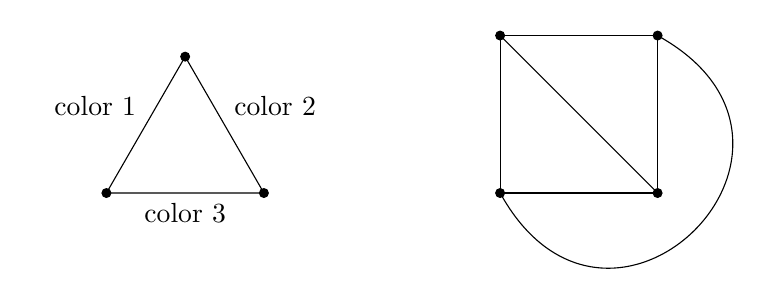
\begin{tikzpicture}
		\clip (-1, -1) rectangle (8, 2.1);
		
		\node[circ] (n1) at (0, 0) {};
		\node[circ] (n2) at (1, {sqrt(3)}) {};
		\node[circ] (n3) at (2, 0) {};
		\draw (n1) -- node[above left] {color 1} (n2)
		-- node[above right] {color 2} (n3)
		-- node[below] {color 3} (n1);
		
		\node[circ] (m1) at (5, 0) {};
		\node[circ] (m2) at (5, 2) {};
		\node[circ] (m3) at (7, 2) {};
		\node[circ] (m4) at (7, 0) {};
		\draw (m1) -- (m2) -- (m3) -- (m4) -- (m1);
		\draw (m2) -- (m4);
		\draw (m1) edge[out=-60, in=-30, looseness=2.5] (m3);
	\end{tikzpicture}
\end{center}
\captionof{figure}{Depictions of an edge coloured graph, and a 4 vertex complete graph.}

\begin{hw}
	Show that the 4 vertex complete graph above can be 3 edge colored. (Use the numbers $1,2,3$ for colors. A figure is shown on the right.)
\end{hw}
\begin{solution}
	Below, we illustrate how the complete 4 vertex graph can be 3 edge coloured: 
	\begin{center}
		\begin{tikzpicture}
			\node[circ] (m1) at (0, 0) {};
			\node[circ] (m2) at (0, 2) {};
			\node[circ] (m3) at (2, 2) {};
			\node[circ] (m4) at (2, 0) {};
			\draw[color=red] (m1) -- node[above left] {1} (m2);
			\draw (m2) -- node[above] {2} (m3);
			\draw[color=red] (m3) -- node[above right] {1} (m4);
			\draw (m4) -- node[below] {2} (m1);
			\draw[color=blue] (m2) -- node[above right] {3} (m4);
			\draw[color=blue] (m1) edge[out=-60, in=-30, looseness=2.5] node[below right] {3} (m3);
		\end{tikzpicture}
	\end{center}
\captionof{figure}{Diagram illustrating how to 3 edge colour the 4 vertex complete graph}
\end{solution}

\begin{hw}
	Prove that any graph with maximum degree $d \geq 1$ can be edge coloured with $2d-1$ colours. 
\end{hw}
\begin{solution}
	We shall proceed by induction on $e$, where $e$ is the number of edges of the graph $G$.
	
	\textbf{\underline{Base Case}}: We observe that for $e=1$, the graph's maximum degree is 1. Now, we can colour the edge red and observe that $G$ is edge coloured with $2(1)-1=1$ colour.
	
	\textbf{\underline{Induction Hypothesis}}: Suppose that our claim holds for $e=k$.
	
	\textbf{\underline{Inductive Step}}: Suppose that a graph $G$, it has $e=k+1$ edges, and has maximum degree $d$. Now, let us remove an edge, leaving us with a graph $G'$ with $k$ edges. By our induction hypothesis, we see that the graph can be $2k-1$ edge coloured, as no vertex has a degree greater than $k$. Now, let us add back in the edges. We see that after adding back in the edge, it must be connected to vertices who are incident to at most $d-1$ other edges. Then, we observe that we at most, we can't use $2(d-1)=2d-2$ colours, thus meaning that we can still colour $G$ using $2d-1$.
	
	Then, by mathematical induction, we can conclude that any graph with maximum degree $d \geq 1$ can be edge coloured with $2d-1$ colours.
\end{solution}

\begin{hw}
	Show that a tree can be edge coloured with $d$ colours where $d$ is the maximum degree of any vertex.
\end{hw}
\begin{solution}
	We shall proceed by induction on $v$, where $v$ is the number of vertices of some tree $T$.
	
	\textbf{\underline{Base Case}}: We see that for $v=1$, the maximum degree of $T$ is 0, and is edge coloured with 0 colours (since it has no edges). Thus, our claim holds for $v=1$.
	
	\textbf{\underline{Induction Hypothesis}}: Suppose that our claim holds for $v=k$.
	
	\textbf{\underline{Inductive Step}}: Now, we want to show that our claim holds for a tree $T$ with $v=k+1$ vertices, whose maximum degree is $d$. First, let us remove one of the leaves, leaving us with a tree $T'$. From here, we observe that, by our induction hypothesis, the tree can be coloured with $d$ colours. Now, let us add back in the leaf. We observe that the leaf must have been connected to a vertex whose degree was at most $d-1$ after the removal. Then, we see that we can't use at most $d-1$ colours to colour the edge, meaning there's still one colour available for use. Thus we can colour $T$ using $d$ colours.
	
	Therefore, by mathematical induction, we can conclude that our claim holds true.
\end{solution}

\newpage

\section{Modular Practice}
Solve the following modular arithmetic equations for $x$ and $y$.

\begin{hw}
	$9x + 5 \equiv 7 \Mod {13}$
\end{hw}
\begin{solution}
	Using rules of modular arithmetic, we observe the following:
	\begin{equation*}
		9x + 5 \equiv 7 \Mod{13} \implies 9x \equiv 2 \Mod{13}
	\end{equation*}

	From here, we observe that $3$ is the multiplicative inverse of $9$, yielding us:
	\begin{equation*}
		(3)9x \equiv (3)2 \Mod{13} \implies x \equiv 6 \Mod{13}
	\end{equation*}
\end{solution}

\begin{hw}
	Show that $3x + 12 \equiv 4 \Mod{21}$ does not have a solution.
\end{hw}
\begin{solution}
	We first see that $3x + 12 \equiv 4 \Mod{21} \implies 3x \equiv 13 \Mod{21}$. Now, for the equation to have a solution, $\gcd{3, 13} \mid 21$. However, we see that $\gcd{3, 13} = 1$, which isn't divisible by 21. Thus, we see that the congruence equation doesn't have a solution.
\end{solution}

\begin{hw}
	Solve the following system of simultaneous equations:
	
	\begin{align*}
		5x + 4y &\equiv 0 \Mod{7} \\
		2x + y &\equiv 4 \Mod{7}
	\end{align*}
\end{hw}
\begin{solution}
	We can rewrite the system of equation as $7x + 5y \equiv 4 \Mod{7}$, or simply $5y \equiv 4 \Mod{7}$. We observe then that $3(5) \equiv 1 \Mod{7}$. So, $3(5y) \equiv 3(4) \Mod{7}$, or simply $y \equiv 5 \Mod{7}$.
	
	Then, plugging this into the second equation in the system, we have that $2x + 5 \equiv 4 \Mod{7}$, which becomes $2x \equiv -1 \Mod{7}$, or in other words $2x \equiv 6 \Mod{7}$. Then, we see that $x \equiv 3 \Mod{7}$.
	
	Therefore, we have that $x \equiv 3 \Mod{7}$ and $y \equiv 5 \Mod{7}$.
\end{solution}

\begin{hw}
	$13^{2023} \equiv x \Mod{12}$
\end{hw}
\begin{solution}
	We observe that $13 \equiv 1 \Mod{12}$. So, we have that $13^{2023} \equiv 1^{2023} \equiv 1 \Mod{12}$. So, $x \equiv 1 \Mod{12}$.
\end{solution}

\begin{hw}
	$7^{62} \equiv x \pmod{11}$
\end{hw}
\begin{solution}
	We observe that, by Fermat's Little Theorem, $7^{10} \equiv 1 \Mod{11}$. So, $7^{62} \equiv 7^{2} \Mod{11}$. From here, $49 \equiv 5 \Mod{11}$. So, $x \equiv 5 \Mod{11}$.
\end{solution}

\newpage

\section{Nontrivial Modular Solutions}
\begin{hw}
	What are all the possible perfect cubes modulo 7?
\end{hw}
\begin{solution}
	We shall proceed by direct proof.
	
	We first observe that, by Fermat's Little Theorem, we have that $n^{7} \equiv n \Mod{7}$. Then, we get that $n^{7} - n \equiv \Mod{7}$.
	
	With this in mind, we observe the following:
	\begin{align*}
		n^{7} - n \equiv 0 \Mod{7} &\implies n(n^{6} - 1) \equiv 0 \Mod{7}\\
		&\implies n(n^{3}+1)(n^{3}-1) \equiv 0 \Mod{7}
	\end{align*}

	Now, we see that in order for this to be true, then $n$, $(n^{3}+1)$, or $(n^{3} -1)$ has to be equal to zero.
	
	Then, we see that there are three cases:
	\begin{itemize}
		\item For $n$ to be zero, then $n=0$.
		\item For $n^{3}-1$ to be zero, then $n=1$
		\item For $n^{3}+1$ to be zero, then $n=-1$
	\end{itemize}

	Then, from here, we can observe the following:
	\begin{align*}
		n = 0 &\implies n^{3} = 0 \\
		n = 1 &\implies n^{3} = 1 \\
		n = -1 &\implies n^{3} = -1
	\end{align*}

	Thus, we have that $n^{3} \equiv 0 \Mod{7}$, $n^{3} \equiv 1 \Mod{7}$, or $n^{3} \equiv 6 \Mod{7}$. So, all the possible perfect cubes modulo $7$ are $0$, $1$, and $6$.
\end{solution}

\begin{hw}
	Show that any solution to $x^3 + 2y^3 \equiv 0 \pmod{7}$ must satisfy $x \equiv y \equiv 0 \pmod{7}$.
\end{hw}
\begin{solution}
%	We observe that as $n^{3} \equiv 0 \Mod{7}$, $n^{3} \equiv 1 \Mod{7}$, or $n^{3} \equiv 6 \Mod{7}$, then we see that the only way for $x^{3} + 2x^{3} \equiv 0 \pmod 7$ is that $x$ and $y$ are both equivalent to $0 \Mod{7}$.
%	
%	Observe that as $n^{3}$ is either equivalent to $0 \Mod{7}$, $1 \Mod{7}$, or $6 \Mod{7}$, then we observe that $x^{3} + 2y^{3}$ can be one of the following:
%	\begin{itemize}
%		\item $0 \pmod 7$ for $x \equiv 0 \pmod 7$ and $y \equiv 0 \pmod 7$
%		\item $2 \pmod 7$ for $x \equiv 0 \pmod 7$ and $y \equiv 1 \pmod 7$
%		\item $5 \pmod 7$ for $x \equiv 0 \pmod 7$ and $y \equiv 6 \pmod 7$
%		
%		\item $1 \Mod{7}$ for $x \equiv 6 \pmod 7$ and $y \equiv 1 \pmod 7$
%		\item $1 \pmod 7$ for $x \equiv 1 \pmod 7$ and $y \equiv 6 \pmod 7$
%	\end{itemize}
%
%	Note that $(n,m)$ represents $x \equiv n \pmod 7$ and $y \equiv m \pmod 7$.
%	
	We shall proceed by direct proof.
	
	Observe that as $n^{3}$ is either equivalent to $0 \Mod{7}$, $1 \Mod{7}$, or $6 \Mod{7}$, which implies the following:
	\begin{itemize}
		\item For $n \equiv 0 \pmod 7$, $2n^{3} \equiv 0 \pmod 7$
		\item For $n \equiv 1 \pmod 7$, $2n^{3} \equiv 2 \pmod 7$
		\item For $n \equiv 6 \pmod 7$, $2n^{3} \equiv 5 \pmod 7$
	\end{itemize}

	From here, by inspection we can see that the only combination that yields us $0 \pmod 7$ is if $x \equiv 0 \pmod 7$ and $y \equiv 0 \pmod 7$.
\end{solution}
\begin{hw}
	Using Problem 6.2, prove that $x^3 + 2y^3 = 7x^2 y$ has no non-trivial solutions $(x, y)$ in the integers. In other words, there are no integers $x$ and $y$, that satisfy this equation, except the trivial solution $x=y=0$.
\end{hw}
\begin{solution}
	We shall proceed by contradiction.
	
	Suppose for contradiction that $x^{3} + 2y^{3} = 7x^{2}y$ has a non-trivial solution for $(x,y)$ with smallest value $\lvert x \rvert$. Now, we have two cases as follow:
	\begin{itemize}
		\item $\lvert x \rvert = 0$
		\item $\lvert x \rvert > 0$
	\end{itemize}

	In the first case, we observe that if $\lvert x \rvert = 0$ then we have:
	\begin{align*}
		(0)^{3} + 2y^{3} &= 7(0)^{2}y \\
		2y^{3} &= 0 \\
		y &= 0
	\end{align*}

	However, this yields us the trivial solution of $(x,y) = (0,0)$, which is a contradiction.
	
	Now, for $\lvert x \rvert > 0$, we know that since $x^{3} + 2y^{3} = 7x^{2}y$, then $x^{3} + 2y^{3} \equiv 0 \pmod 7$.
	
	From here, we observe that the only values that satisfies this is for both $x,y \equiv 0 \pmod 7$. Now, as we assumed that there is some non-trivial solution to the equation, then let $x = 7a$ and $y = 7b$, where $a,b \not= 0$, be the smallest solution to our equation. From here, we then observe the following:
	\begin{align*}
		x^{3} + 2y^{3} &= 7x^{3}y \\
		(7a)^{3} + 2(7b)^{3} &= 7(7a)^{2}(7b) \\
		a^{3} + 2b^{3} &= 7a^{2}b
	\end{align*}

	However, from here we notice that we now have that $a^{3} + 2b^{3} = 7a^{2}b$. But, we now have that $\lvert a \rvert < \lvert x \rvert$, which is a contradiction.
	
	Therefore, the only solution to the equation is the trivial solution.
\end{solution}

\newpage

\section{Wilson's Theorem}
\begin{hw}
	Wilson's Theorem states the following is true if and only if $p$ is prime:
	\[(p - 1)! \equiv -1 \pmod{p}.\]
	Prove both directions (it holds if AND only if $p$ is prime).
\end{hw}
\begin{solution}
	In order to prove Wilson's Theorem, we have to prove the claim in both directions. To begin with, let us start with the forward direction.
	
	\begin{proof}[If] We shall proceed by cases.
		
		Suppose that $p$ is prime.
		
		To begin with, we want to show that for $p=2$, our claim holds true. In this case, we see that $(2-1)! \equiv 1 \equiv -1 \pmod 2$. Thus, our claim holds for $p=2$.
		
		Now, for $p>2$, we observe that $(p-1)! = (p-1)(p-2) \ldots (2)(1)$. Now, observe that since $p$ is prime, it means that all the integers in $(p-1)!$ must be relatively prime to $p$. Then, for each of these integers $m$, there are two cases:
		\begin{itemize}
			\item There's another integer $n$ such that $mn \equiv 1 \Mod{p}$. In other words, every $m$ has an inverse $n$.
			
			\item The number is a self-inverse.
		\end{itemize}
	
		In the second case, we observe that finding self-inverses is equivalent to solving for $m^{2} \equiv 1 \pmod p$. We can rearrange it to get that $m^{2} - 1 = (m+1)(m-1) \equiv 0 \pmod p$. In this case, the only two solutions are $m \equiv \pm 1 \pmod p$. In other words, $m_{1} = 1 \equiv 1 \pmod p$ and $m_{2} = p-1 \equiv -1 \pmod p$.
		
		Now, we know that since $p$ is prime, and $p>2$, it must be an odd number. Then, there are an even number of terms for $(p-1)!$. After excluding $1$ and $p-1$ (the self-inverses), we can start pairing up each term with their inverses. In other words, we have that $(p-2)! \equiv 1 \pmod p$.
		
		Thus, we have that $(p-1)! \equiv (p-1)(p-2)! \equiv (p-1)(1) \equiv -1 \Mod{p}$.
		
		Therefore, if $p$ is prime then we have that $(p-1)! \equiv -1 \pmod p$.
	\end{proof}

	\begin{proof}[Only if]
		We shall proceed by contradiction.
		
		Suppose for contradiction that $(p-1)! \equiv -1 \Mod{p}$ for some composite $p$. 
		
		As $p$ is composite, we see that $p=qr$, where $q$ is a prime factor of $p$. From here, we observe that since $q$ is a prime factor of $p$, then $q \leq p-1$. This then implies that $(p-1)! \equiv 0 \pmod q$ as $(p-1)!$ must contain $q$. In other words, $q$ divides $(p-1)!$.
		
		Now, by our assumption, we said that $(p-1)! \equiv -1 \pmod p$. Then, this means the following:
		\begin{align*}
			(p-1)! \equiv -1 \pmod p &\implies (p-1)! = pk - 1 \tag{for $k \in \ZZ$} \\
			&\implies (p-1)! = (qr)k - 1 \\
			&\implies (p-1)! = q(rk) - 1 \\
			&\implies (p-1)! \equiv -1 \pmod q 
		\end{align*} 
	
		However, we see that this contradicts with the fact that $(p-1)! \equiv 0 \pmod q$. Therefore, we can conclude that for $(p-1)! \equiv -1 \pmod p$, $p$ must be prime.
	\end{proof}

	Since we have proven our claim in both directions, we can thus conclude that Wilson's Theorem is true.
\end{solution}
\end{document}